\documentclass[border=2pt]{standalone}
% Shared style for the vector figures (Figs. 1, 2, 4). Compile each fig*.tex with pdflatex.
\usepackage[T1]{fontenc}
\usepackage{lmodern}
\usepackage{amsmath,amssymb}
\usepackage{sansmath}
\usepackage{tikz}
\usetikzlibrary{arrows.meta,calc,positioning,fit,patterns,decorations.pathreplacing}
\renewcommand{\familydefault}{\sfdefault}
\sansmath
% class colours (blue, green, orange, purple, grey): distinguishable in greyscale by label, not by colour alone
\definecolor{cD}{HTML}{1F5FAE}
\definecolor{cL}{HTML}{1B7F4B}
\definecolor{cP}{HTML}{C2590F}
\definecolor{cG}{HTML}{6A3D9A}
\definecolor{cH}{HTML}{4D4D4D}
\definecolor{cA}{HTML}{8A5A00}   % PPA (event audit)
\definecolor{ink}{HTML}{1A1A1A}
\definecolor{rule}{HTML}{8C8C8C}
\tikzset{
  >={Stealth[length=5pt,width=4pt]},
  every picture/.style={line cap=round,line join=round,text=ink},
  box/.style={draw=#1,line width=0.7pt,rounded corners=2.5pt,fill=#1!7,align=center,inner sep=3pt},
  plain/.style={draw=rule,line width=0.6pt,rounded corners=2.5pt,fill=white,align=center,inner sep=3pt},
  flow/.style={->,line width=0.6pt,draw=ink!85},
}
\hyphenpenalty=10000\exhyphenpenalty=10000

\begin{document}
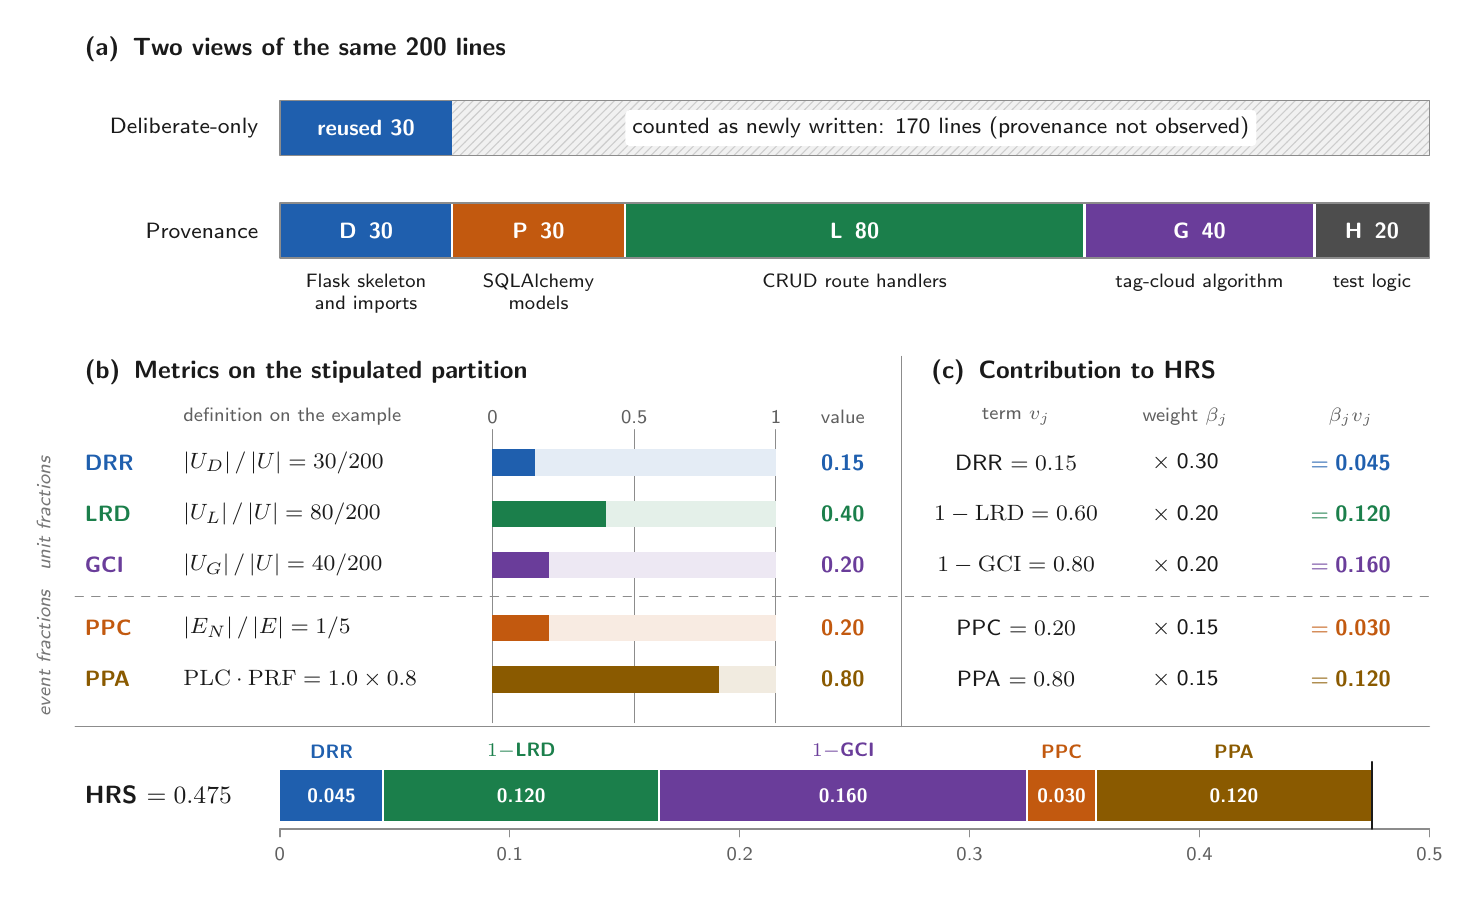
\begin{tikzpicture}[x=1cm,y=1cm]
% =================== (a) two views of the same 200 lines ===================
\node[anchor=west,font=\small\bfseries] at (0,0.05) {(a)\enspace Two views of the same 200 lines};
% scale: 200 lines = 14.6 cm, bars start at x = 2.6
\def\xo{2.6}\def\s{0.073}
% --- deliberate-only view
\node[anchor=east,font=\footnotesize,align=right,text width=2.4cm] at (\xo-0.15,-0.95) {Deliberate-only};
\fill[cD] (\xo,-0.6) rectangle (\xo+30*\s,-1.3);
\node[text=white,font=\footnotesize\bfseries] at (\xo+15*\s,-0.95) {reused 30};
\fill[ink!6] (\xo+30*\s,-0.6) rectangle (\xo+200*\s,-1.3);
\fill[pattern=north east lines,pattern color=ink!22] (\xo+30*\s,-0.6) rectangle (\xo+200*\s,-1.3);
\draw[rule,line width=0.5pt] (\xo,-0.6) rectangle (\xo+200*\s,-1.3);
\node[font=\footnotesize,fill=white,inner sep=2.5pt,rounded corners=1.5pt] at (\xo+115*\s,-0.95) {counted as newly written: 170 lines (provenance not observed)};
% --- provenance view
\node[anchor=east,font=\footnotesize,align=right,text width=2.4cm] at (\xo-0.15,-2.25) {Provenance};
\newcommand{\seg}[6]{% from, to, colour, letter, lines, description
  \fill[#3] (\xo+#1*\s,-1.9) rectangle (\xo+#2*\s,-2.6);
  \pgfmathsetmacro{\xm}{\xo+0.5*(#1+#2)*\s}
  \pgfmathsetmacro{\tw}{(#2-#1)*\s-0.12}
  \node[text=white,font=\footnotesize\bfseries] at (\xm,-2.25) {#4\enspace #5};
  \node[font=\scriptsize,align=center,text width=\tw cm,anchor=north] at (\xm,-2.68) {#6};}
\seg{0}{30}{cD}{D}{30}{Flask skeleton and imports}
\seg{30}{60}{cP}{P}{30}{SQLAlchemy models}
\seg{60}{140}{cL}{L}{80}{CRUD route handlers}
\seg{140}{180}{cG}{G}{40}{tag-cloud algorithm}
\seg{180}{200}{cH}{H}{20}{test logic}
\foreach \v in {30,60,140,180} \draw[white,line width=0.8pt] (\xo+\v*\s,-1.9) -- (\xo+\v*\s,-2.6);
\draw[rule,line width=0.5pt] (\xo,-1.9) rectangle (\xo+200*\s,-2.6);

% =================== (b) metrics, (c) contributions ===================
\node[anchor=west,font=\small\bfseries] at (0,-4.05) {(b)\enspace Metrics on the stipulated partition};
\node[anchor=west,font=\small\bfseries] at (10.75,-4.05) {(c)\enspace Contribution to HRS};
\draw[rule,line width=0.4pt] (10.5,-3.85) -- (10.5,-8.55);
% column heads
\node[anchor=west,font=\scriptsize,text=ink!70] at (1.25,-4.62) {definition on the example};
\node[font=\scriptsize,text=ink!70] at (9.75,-4.62) {value};
\node[font=\scriptsize,text=ink!70] at (11.95,-4.62) {term $v_j$};
\node[font=\scriptsize,text=ink!70] at (14.1,-4.62) {weight $\beta_j$};
\node[font=\scriptsize,text=ink!70] at (16.2,-4.62) {$\beta_j v_j$};
% bar scale 0..1 over 3.6 cm starting at x = 5.3
\def\bx{5.3}\def\bw{3.6}
\foreach \t/\l in {0/0,0.5/0.5,1/1}{
  \draw[rule,line width=0.4pt] (\bx+\t*\bw,-4.78) -- (\bx+\t*\bw,-8.5);
  \node[font=\scriptsize,text=ink!70] at (\bx+\t*\bw,-4.62) {\l};}
\newcommand{\mrow}[8]{% y, colour, acronym, definition, value, term text, weight, contribution
  \node[anchor=west,font=\footnotesize\bfseries,text=#2] at (0,#1) {#3};
  \node[anchor=west,font=\footnotesize] at (1.25,#1) {#4};
  \fill[#2!12] (\bx,#1-0.17) rectangle (\bx+\bw,#1+0.17);
  \fill[#2] (\bx,#1-0.17) rectangle (\bx+#5*\bw,#1+0.17);
  \node[font=\footnotesize\bfseries,text=#2] at (9.75,#1) {#5};
  \node[font=\footnotesize] at (11.95,#1) {#6};
  \node[font=\footnotesize] at (14.1,#1) {$\times\;$#7};
  \node[font=\footnotesize\bfseries,text=#2] at (16.2,#1) {$=\;$#8};}
\mrow{-5.20}{cD}{DRR}{$|U_D|\,/\,|U| = 30/200$}{0.15}{DRR $= 0.15$}{0.30}{0.045}
\mrow{-5.85}{cL}{LRD}{$|U_L|\,/\,|U| = 80/200$}{0.40}{$1-\mathrm{LRD} = 0.60$}{0.20}{0.120}
\mrow{-6.50}{cG}{GCI}{$|U_G|\,/\,|U| = 40/200$}{0.20}{$1-\mathrm{GCI} = 0.80$}{0.20}{0.160}
\draw[rule,dashed,line width=0.4pt] (0,-6.90) -- (17.2,-6.90);
\mrow{-7.30}{cP}{PPC}{$|E_N|\,/\,|E| = 1/5$}{0.20}{PPC $= 0.20$}{0.15}{0.030}
\mrow{-7.95}{cA}{PPA}{$\mathrm{PLC}\cdot\mathrm{PRF} = 1.0 \times 0.8$}{0.80}{PPA $= 0.80$}{0.15}{0.120}
\node[rotate=90,font=\scriptsize\itshape,text=ink!60] at (-0.4,-5.85) {unit fractions};
\node[rotate=90,font=\scriptsize\itshape,text=ink!60] at (-0.4,-7.62) {event fractions};

% =================== HRS as a stacked sum ===================
\draw[rule,line width=0.4pt] (0,-8.55) -- (17.2,-8.55);
\node[anchor=west,font=\small\bfseries,align=left] at (0,-9.42) {HRS $= 0.475$};
% scale: 0..0.5 over 14.6 cm
\def\hs{29.2}
\newcommand{\hseg}[5]{% from, to, colour, value label, acronym
  \fill[#3] (\xo+#1*\hs,-9.1) rectangle (\xo+#2*\hs,-9.75);
  \pgfmathsetmacro{\xm}{\xo+0.5*(#1+#2)*\hs}
  \node[text=white,font=\scriptsize\bfseries] at (\xm,-9.425) {#4};
  \node[font=\scriptsize\bfseries,text=#3,anchor=south] at (\xm,-9.08) {#5};}
\hseg{0}{0.045}{cD}{0.045}{DRR}
\hseg{0.045}{0.165}{cL}{0.120}{$1-$LRD}
\hseg{0.165}{0.325}{cG}{0.160}{$1-$GCI}
\hseg{0.325}{0.355}{cP}{0.030}{PPC}
\hseg{0.355}{0.475}{cA}{0.120}{PPA}
\foreach \v in {0.045,0.165,0.325,0.355} \draw[white,line width=0.8pt] (\xo+\v*\hs,-9.1) -- (\xo+\v*\hs,-9.75);
\draw[rule,line width=0.5pt] (\xo,-9.85) -- (\xo+0.5*\hs,-9.85);
\foreach \t in {0,0.1,0.2,0.3,0.4,0.5}{
  \draw[rule,line width=0.5pt] (\xo+\t*\hs,-9.85) -- (\xo+\t*\hs,-9.95);
  \node[font=\scriptsize,text=ink!70,anchor=north] at (\xo+\t*\hs,-9.97) {\t};}
\draw[ink,line width=0.7pt] (\xo+0.475*\hs,-9.0) -- (\xo+0.475*\hs,-9.85);
\end{tikzpicture}
\end{document}
